\section{Generalization to \texorpdfstring{$N_{\mathrm s}$}{Ns} strings}
\label{sec:n-string-generalization}

We now generalize the preceding calculation to $N_{\mathrm s}$ independent
Nambu--Goto strings with equal tension $T$.  The label
$A=1,\ldots,N_{\mathrm s}$ counts strings, while
$i=1,\ldots,n_\perp$ counts transverse components,
with $n_\perp=D-2$.  Keeping these two multiplicities distinct is essential:
$N_{\mathrm s}$ is not the $N$ used for the number of massive components in
the two-string calculation above.

Through four-derivative order, the common-worldsheet Minkowski Lagrangian is
\begin{align}
  \mathcal L_{N_{\mathrm s}}
  ={}&-N_{\mathrm s}T
  -\frac{T}{2}\sum_{A=1}^{N_{\mathrm s}}
    \partial_aX_A^i\partial^aX_A^i
  -\frac{T}{8}\sum_{A=1}^{N_{\mathrm s}}
    \left(\partial_aX_A^i\partial^aX_A^i\right)^2
  \notag\\
  &+\frac{T}{4}\sum_{A=1}^{N_{\mathrm s}}
    \left(\partial_aX_A^i\partial_bX_A^i\right)
    \left(\partial^aX_A^j\partial^bX_A^j\right)
  +\mathcal O(\partial^6).
  \label{eq:n-string-ng-four-derivative}
\end{align}

\subsection{Center-of-mass and relative modes}

Let $O$ be an $N_{\mathrm s}\times N_{\mathrm s}$ orthogonal matrix whose
first column is constant,
\begin{align}
  X_A^i&=\sum_{\alpha=0}^{N_{\mathrm s}-1}O_{A\alpha}Y_\alpha^i,
  &O_{A0}&=\frac{1}{\sqrt{N_{\mathrm s}}},
  &\sum_AO_{A\alpha}O_{A\beta}&=\delta_{\alpha\beta}.
  \label{eq:n-string-orthogonal-transform}
\end{align}
Thus
\begin{equation}
  Y_0^i=\frac{1}{\sqrt{N_{\mathrm s}}}
        \sum_{A=1}^{N_{\mathrm s}}X_A^i
  \label{eq:n-string-normalized-center-mode}
\end{equation}
is the normalized center-of-mass mode, and
$Y_r^i$, $r=1,\ldots,N_{\mathrm s}-1$, are any orthonormal basis for the
relative subspace.  Physical results cannot depend on the particular choice
of those last $N_{\mathrm s}-1$ columns of $O$.

As in the two-string calculation, the mass deformation is additional physics,
not a consequence of the shift-symmetric Nambu--Goto action.  We choose the
permutation-symmetric deformation that gives every relative mode the same mass
$m$ while leaving $Y_0$ massless:
\begin{align}
  \Delta\mathcal L_m
  &=-\frac{Tm^2}{2}\sum_{r=1}^{N_{\mathrm s}-1}Y_r^iY_r^i
  \notag\\
  &=-\frac{Tm^2}{2N_{\mathrm s}}
    \sum_{A<B}(X_A^i-X_B^i)(X_A^i-X_B^i).
  \label{eq:n-string-relative-mass-deformation}
\end{align}
The equality follows from
$\sum_{A<B}(X_A-X_B)^2=N_{\mathrm s}\sum_AX_A^2-(\sum_AX_A)^2$.
For $N_{\mathrm s}=2$, Eq.~\eqref{eq:n-string-relative-mass-deformation}
reduces to $-Tm^2(X_1-X_2)^2/4$, exactly
Eq.~\eqref{eq:relative-mass-term}.

The orthonormal modes have the canonical normalization
\begin{equation}
  \phi_\alpha^i=\sqrt{T}\,Y_\alpha^i,
  \label{eq:n-string-canonical-fields}
\end{equation}
so their quadratic Minkowski Lagrangian is
\begin{align}
  \mathcal L_2={}&-\frac12\partial_a\phi_0^i\partial^a\phi_0^i
  -\frac12\sum_{r=1}^{N_{\mathrm s}-1}
    \left(\partial_a\phi_r^i\partial^a\phi_r^i
          +m^2\phi_r^i\phi_r^i\right).
  \label{eq:n-string-quadratic-canonical}
\end{align}

\begin{figure}[h!]
  \centering
  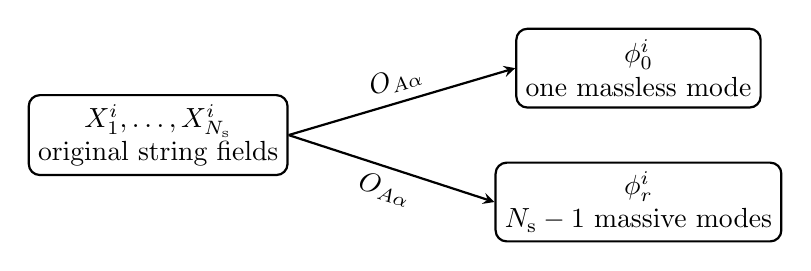
\begin{tikzpicture}[line width=0.8pt,>=stealth]
    \node[draw,rounded corners,align=center,minimum width=3.0cm,
      minimum height=1.0cm] (original) at (-3.2,0)
      {$X_1^i,\ldots,X_{N_{\mathrm s}}^i$\\original string fields};
    \node[draw,rounded corners,align=center,minimum width=2.6cm,
      minimum height=1.0cm] (center) at (2.9,0.85)
      {$\phi_0^i$\\one massless mode};
    \node[draw,rounded corners,align=center,minimum width=2.6cm,
      minimum height=1.0cm] (relative) at (2.9,-0.85)
      {$\phi_r^i$\\$N_{\mathrm s}-1$ massive modes};
    \draw[->] (original.east) -- node[above,sloped] {$O_{A\alpha}$}
      (center.west);
    \draw[->] (original.east) -- node[below,sloped] {$O_{A\alpha}$}
      (relative.west);
  \end{tikzpicture}
  \caption{Orthogonal decomposition of $N_{\mathrm s}$ equal-tension string
  fluctuations.  Each mode also carries $n_\perp$ transverse components.}
  \label{fig:n-string-mode-decomposition}
\end{figure}

\subsection{Quartic interaction and the relative projector}

Define the canonically normalized field attached to the original string
label, $\Phi_A^i\equiv\sqrt{T}X_A^i=\sum_\alpha O_{A\alpha}\phi_\alpha^i$.
The Wick-rotated quartic interaction is
\begin{align}
  \mathcal L_{4,E}
  ={}&\frac{1}{8T}\sum_A
    \left(\partial_a\Phi_A^i\partial_a\Phi_A^i\right)^2
  \notag\\
  &-\frac{1}{4T}\sum_A
    \left(\partial_a\Phi_A^i\partial_b\Phi_A^i\right)
    \left(\partial_a\Phi_A^j\partial_b\Phi_A^j\right).
  \label{eq:n-string-quartic-euclidean}
\end{align}
On an infinite flat worldsheet, every center-of-mass loop is scaleless in
dimensional regularization.  Therefore only the massive relative part is
needed for the vacuum figure-eight.  Introduce
\begin{equation}
  R_A^i\equiv\sum_{r=1}^{N_{\mathrm s}-1}O_{Ar}\phi_r^i,
  \qquad
  P_{AB}\equiv\sum_{r=1}^{N_{\mathrm s}-1}O_{Ar}O_{Br}
  =\delta_{AB}-\frac{1}{N_{\mathrm s}}.
  \label{eq:n-string-relative-field-projector}
\end{equation}
The matrix $P$ is the basis-independent orthogonal projector onto the relative
subspace: $P^2=P$ and $\sum_BP_{AB}=0$.  Its diagonal elements obey
\begin{equation}
  P_{AA}=\frac{N_{\mathrm s}-1}{N_{\mathrm s}},
  \qquad
  \sum_AP_{AA}^2=\frac{(N_{\mathrm s}-1)^2}{N_{\mathrm s}}.
  \label{eq:n-string-projector-diagonal-factor}
\end{equation}

The massive propagator and its coincident derivative contraction are
\begin{align}
  \langle R_A^i(p)R_B^j(-p)\rangle_0
  &=\frac{\delta^{ij}P_{AB}}{p^2+m^2},
  \notag\\
  \left\langle\partial_aR_A^i\partial_bR_B^j\right\rangle_0
  &=\delta^{ij}\delta_{ab}P_{AB}\frac{K_m}{d}.
  \label{eq:n-string-relative-derivative-propagator}
\end{align}
For each fixed $A$, let
\begin{equation}
  \mathcal A_A\equiv\partial_aR_A^i\partial_aR_A^i,
  \qquad
  \mathcal B_A\equiv
  (\partial_aR_A^i\partial_bR_A^i)
  (\partial_aR_A^j\partial_bR_A^j).
\end{equation}
The same three Wick pairings displayed in
Eqs.~\eqref{eq:A2-wick-result} and \eqref{eq:B-wick-result} now give
\begin{align}
  \langle\mathcal A_A^2\rangle_0
  &=P_{AA}^2\frac{n_\perp(n_\perp d+2)}{d}K_m^2,
  \notag\\
  \langle\mathcal B_A\rangle_0
  &=P_{AA}^2\frac{n_\perp(n_\perp+d+1)}{d}K_m^2.
  \label{eq:n-string-wick-pairings}
\end{align}
Explicitly, the three terms for $\mathcal A_A^2$ are
$P_{AA}^2K_m^2\{n_\perp^2,n_\perp/d,n_\perp/d\}$, while those for
$\mathcal B_A$ are
$P_{AA}^2K_m^2\{n_\perp^2/d,n_\perp,n_\perp/d\}$.  Thus no contraction or
diagrammatic symmetry factor is hidden in Eq.~\eqref{eq:n-string-wick-pairings}.

The vacuum-diagram topologies remain those of
Fig.~\ref{fig:vacuum-diagrams}: the Gaussian circle carries a relative label
$r=1,\ldots,N_{\mathrm s}-1$ and a transverse label
$i=1,\ldots,n_\perp$, while the figure-eight contains the relative-projector
weights in Eq.~\eqref{eq:n-string-projector-diagonal-factor}.  Combining the
two quartic operators gives
\begin{align}
  \Delta\rho_{\mathrm{fig8}}^{(N_{\mathrm s})}
  &=\frac{1}{8T}\sum_A\langle\mathcal A_A^2\rangle_0
    -\frac{1}{4T}\sum_A\langle\mathcal B_A\rangle_0
  \notag\\
  &=\boxed{
    \frac{n_\perp(N_{\mathrm s}-1)^2}{8TN_{\mathrm s}d}
    \left[n_\perp(d-2)-2d\right]K_m^2 }.
  \label{eq:n-string-figure-eight-general-d}
\end{align}

\subsection{Dimensional-regularization expansion and collected result}

Set $d=2-2\epsilon$, retain the full $d$ dependence until after multiplying
the divergent loop integrals, and use $K_m=-m^2I_m$ with
Eq.~\eqref{eq:massive-tadpole-dimreg}.  The coefficient of $K_m^2$ expands as
\begin{align}
  &\frac{n_\perp(N_{\mathrm s}-1)^2}{8TN_{\mathrm s}d}
   \left[n_\perp(d-2)-2d\right]
  \notag\\
  &\qquad=-\frac{n_\perp(N_{\mathrm s}-1)^2}{4TN_{\mathrm s}}
   -\frac{n_\perp^2(N_{\mathrm s}-1)^2}{8TN_{\mathrm s}}\epsilon
   -\frac{n_\perp^2(N_{\mathrm s}-1)^2}{8TN_{\mathrm s}}\epsilon^2
   +\mathcal O(\epsilon^3).
  \label{eq:n-string-evanescent-coefficient}
\end{align}
Consequently the bare figure-eight graph through finite order is
\begin{align}
  \Delta\rho_{\mathrm{fig8}}^{(N_{\mathrm s}),\mathrm{bare}}
  =-\frac{n_\perp(N_{\mathrm s}-1)^2m^4}
          {64\pi^2TN_{\mathrm s}}
  \Bigg[
    &\frac{1}{\epsilon^2}
    +\frac{2L+n_\perp/2}{\epsilon}
    +2L^2+\frac{\pi^2}{6}
  \notag\\
    &+n_\perp L+\frac{n_\perp}{2}
    +\mathcal O(\epsilon)
  \Bigg].
  \label{eq:n-string-figure-eight-bare}
\end{align}

There are $n_\perp(N_{\mathrm s}-1)$ real massive fields, so their Gaussian
one-loop contribution after $\overline{\mathrm{MS}}$ subtraction is
\begin{equation}
  \boxed{
  \rho_{1\text{-loop}}^{(N_{\mathrm s}),\overline{\mathrm{MS}}}
  =\frac{n_\perp(N_{\mathrm s}-1)m^2}{8\pi}(1+L) }.
  \label{eq:n-string-gaussian-one-loop}
\end{equation}
Combining the classical energy, the one-loop determinant, and the bare
figure-eight gives
\begin{align}
  \rho_{\mathrm{vac}}^{(N_{\mathrm s})}
  ={}&N_{\mathrm s}T
  +\frac{n_\perp(N_{\mathrm s}-1)m^2}{8\pi}
    \left(\frac{1}{\epsilon}+1+L\right)
  \notag\\
  &-\frac{n_\perp(N_{\mathrm s}-1)^2m^4}
          {64\pi^2TN_{\mathrm s}}
   \left[
    \frac{1}{\epsilon^2}
    +\frac{2L+n_\perp/2}{\epsilon}
    +2L^2+\frac{\pi^2}{6}
    +n_\perp L+\frac{n_\perp}{2}
   \right]
  \notag\\
  &+\delta\rho_{\mathrm{vac}}^{(N_{\mathrm s})}
   +\rho_{\mathrm{param\,ct}}^{(N_{\mathrm s})}
   +\mathcal O(\epsilon)+\mathcal O(T^{-2}).
  \label{eq:n-string-total-vacuum-energy-bare}
\end{align}
If the displayed poles are simply removed and all finite counterterms are set
to zero, the graph-only finite bookkeeping expression is
\begin{align}
  \rho_{\mathrm{vac}}^{(N_{\mathrm s}),\mathrm{graph,fin}}
  ={}&N_{\mathrm s}T
  +\frac{n_\perp(N_{\mathrm s}-1)m^2}{8\pi}(1+L)
  \notag\\
  &-\frac{n_\perp(N_{\mathrm s}-1)^2m^4}
          {64\pi^2TN_{\mathrm s}}
   \left(2L^2+\frac{\pi^2}{6}
         +n_\perp L+\frac{n_\perp}{2}\right)
  +\mathcal O(T^{-2}).
  \label{eq:n-string-total-vacuum-energy-graph-finite}
\end{align}
As before, Eq.~\eqref{eq:n-string-total-vacuum-energy-graph-finite} is not a
scheme-independent physical vacuum energy.  A renormalized result requires a
vacuum-energy/string-tension counterterm and any parameter-counterterm
insertions induced by the additional mass-generating physics.

Several limits provide direct checks.  For $N_{\mathrm s}=1$, the relative
projector vanishes and there are no massive relative-loop contributions.  For
$N_{\mathrm s}=2$, choose
$O=2^{-1/2}\bigl(\begin{smallmatrix}1&1\\1&-1\end{smallmatrix}\bigr)$.
Then $Y_0=X_{\mathrm s}/\sqrt2$, $Y_1=X_{\mathrm r}/\sqrt2$,
$\phi_0=\sqrt{T/2}X_{\mathrm s}$, and
$\phi_1=\sqrt{T/2}X_{\mathrm r}$.  Moreover
$(N_{\mathrm s}-1)^2/N_{\mathrm s}=1/2$, so
Eqs.~\eqref{eq:n-string-figure-eight-general-d} and
\eqref{eq:n-string-figure-eight-bare} reduce exactly to
Eqs.~\eqref{eq:figure-eight-general-d} and
\eqref{eq:figure-eight-bare-expanded} after identifying
$n_\perp=N$.
